\documentclass[12pt]{article}
\usepackage{amsmath}
\usepackage{graphicx}
\usepackage{caption}
\usepackage{subcaption}
 \usepackage[russian]{babel}
\usepackage{booktabs}
\usepackage{float}
\usepackage{minted}
\usepackage{verbatim}
\usepackage[utf8]{inputenc}
\usepackage{geometry}
\usepackage{multirow}
\usepackage{setspace}
\usepackage{parskip}
\usepackage[bottom]{footmisc}
\usepackage{tikz}
\usepackage[section]{placeins}

% This style is used to create block diagrams, you'll find it useful since many of your figures would be of that form, I'll try add more styles in the future :)
\usetikzlibrary{trees,positioning,fit,calc}
\tikzset{block/.style = {draw, fill=blue!20, rectangle,
                         minimum height=3em, minimum width=4em},
        input/.style = {coordinate},
        output/.style = {coordinate}
}

\usepackage[section]{minted}
\usepackage{xcolor}
\usemintedstyle{porland}

\usepackage{chngcntr}
\counterwithin{figure}{section}

\renewcommand{\arraystretch}{1.5}

\usepackage[hidelinks]{hyperref}
\hypersetup{
    linktoc=all
}

\renewcommand\listingscaption{Listing}
\renewcommand\listoflistingscaption{List of Listings}

\usepackage{scrhack}
\usepackage{tocbasic}
\setuptoc{lol}{levelup}

\usepackage{indentfirst}
\geometry{a4paper, margin=1in}

%----------EDIT COVER INFO HERE -----------------%

\def \LOGOPATH {assets/logo3.png}
\def \DEPARTEMENT {Министерство образования и науки Российской Федерации 
Федеральное государственное образовательное учреждение высшего образования
\\ «Национальный исследовательский университет «МЭИ» 
Институт ИВТ
Кафедра ПМИИ
}
\def \REPORTTITLE {Отчет по лабораторной работе номер 4 \\ Windows. Процессы, потоки и волокна. Механизмы синхронизации}
\def \STUDENTNAME {Желтиков Александр Алексеевич}
\def \STUDENTID {STUDNUM}


%------------------------------------------------%

\setlength{\parindent}{2em}
\setlength{\parskip}{0em}

\begin{document}

\pagenumbering{arabic}

\begin{titlepage}
    \vfill
    \begin{center}
        \includegraphics[width=0.7\textwidth]{\LOGOPATH} \\
        \hfill \\
        \Large{\DEPARTEMENT} \\
        \vfill
        \textbf{\LARGE{\REPORTTITLE}}
    \end{center}
    \vfill
    \begin{flushleft}
        \Large{\textbf{Подгтовил:} \STUDENTNAME} \\
        \Large{\textbf{Дата:} \today}
    \end{flushleft}
    \vfill
\end{titlepage}

\clearpage

\newpage
\tableofcontents
\newpage
\section{Цель работы. Лабораторное задание.}

\textit{Изучение техники разработки Win32- приложений и способов согласования работы потоков и различных процессов.} \\

\subsection{Создать приложение Windows и добавить в него код создания нового потока (thread). Отладить и протестировать проект.}

Для начала создадим функцию потока:\\

\begin{minted}[fontsize=\footnotesize]{c}
DWORD WINAPI ThrFunс(LPVOID lparam) {
    EnterCriticalSection(&critSection);
    SetWindowText(Text1, L"1 Поток запущен");
    Sleep(3000);
    LeaveCriticalSection(&critSection);
    SetWindowText(Text1, L"1 Поток завершил свою функцию");
    ExitThread(0);
    return 0;
}
\end{minted}

Затем создадим кнопку для запуска нашего потока\\


\begin{minted}[fontsize=\footnotesize]{c}
// Кнопка для запуска потока
Thr1 = CreateWindow(L"BUTTON", L"Запустить поток",
   WS_BORDER | WS_VISIBLE | WS_CHILD | BS_PUSHBUTTON, 50, 100, 200, 30, 
   hWnd, (HMENU)Thr1ID, hInstance, nullptr);
       
// Обработка события кнопки
case Thr1ID:
    Thread1 = CreateThread(NULL, 0, ThrFunс, NULL, 0, NULL); // Создаем поток
    if (Thread1 == NULL)
    {
        ExitProcess(3);
    }
    break;
\end{minted}

Тестирование:\\
\begin{center}
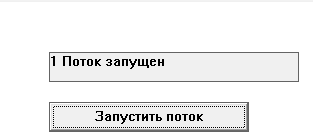
\includegraphics[width=0.7\textwidth]{assets/1.png}\\
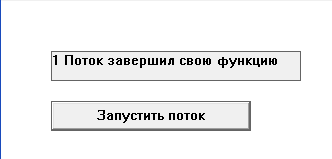
\includegraphics[width=0.7\textwidth]{assets/2.png}\\    
\end{center}

\subsection{Создать два приложения, одно из которых будет ожидать сообщения от второго приложения (и только после этого продолжит свою работу)}

Создадим второе приложение и добавим в него кнопку ожидания сообщения.\\
\begin{minted}[fontsize=\footnotesize]{c}
wait = CreateWindow(L"BUTTON", L"Ожидание сообщения", 
    WS_BORDER | WS_VISIBLE | WS_CHILD | BS_PUSHBUTTON, 
    50, 100, 200, 30, hWnd, (HMENU)waitID, hInstance, nullptr);

// Обработка кнопки
case waitID:
{
    if (!FindWindow(NULL, L"Lab4OS")) {
        MessageBox(Text1, L"Приложение, для отправки сообщения, не найдено!", L"ERROR", MB_ICONEXCLAMATION);
    }
    else {
        SetWindowText(Text1, L"Ожидаем сообщение");
        hEvent = CreateEvent(NULL, TRUE, FALSE, L"Event1");
        if (!hEvent) {
            SetWindowText(Text1, L"К сожалению не удалось создать событие");
        }
        else {
            WaitForSingleObject(hEvent, INFINITE);
            ResetEvent(hEvent);
            SetWindowText(Text1, L"Вроде работает...");
        }
    }
}
\end{minted}

Далее добавим в первое приложение кнопку для отпраки сообщения.

\begin{minted}[fontsize=\footnotesize]{c}
SendEvent = CreateWindow(L"BUTTON", L"Отправить сообщение",
   WS_BORDER | WS_VISIBLE | WS_CHILD | BS_PUSHBUTTON, 
   50, 150, 200, 30, hWnd, (HMENU)SendEventID, hInstance, nullptr);

case SendEventID:
    hEvent = OpenEvent(EVENT_ALL_ACCESS, TRUE, L"Event1");
    if (!hEvent)
        SetWindowText(Text1, L"Не найден получатель сообщения");
    else {
        SetWindowText(Text1, L"Отправлено сообщение");
        SetEvent(hEvent);
    }
    break;
\end{minted}

Если второе приложение не ожидает сообщение от первого, то будет такое сообщение:\\

\begin{center}
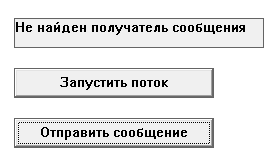
\includegraphics[width=0.7\textwidth]{assets/3.png}\\
\end{center}

Теперь отравим сообщение: \\

\begin{center}
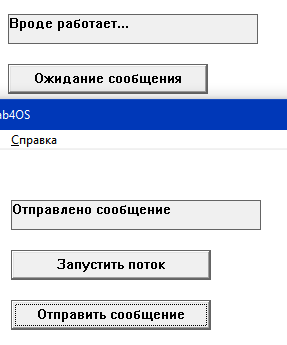
\includegraphics[width=0.7\textwidth]{assets/4.png}\\
\end{center}

Если приложение не запущено и мы будем ожидать сообщение, то выскочит ошибка:\\

\begin{center}
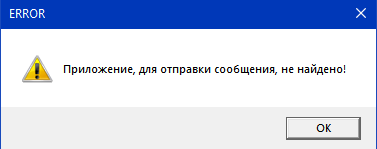
\includegraphics[width=0.7\textwidth]{assets/5.png}\\
\end{center}

\subsection{Добавить в первое приложение код создания объекта синхронизации и код ожидания.}

\textit{\textbf{Сделано в предыдущем пункте!}}\\
\subsection{Добавить во второе приложения требуемые операции и команды работы с объектом синхронизации.}
\textit{\textbf{Смотреть в предыдущий пункт!}}\\
\subsection{Произвести тестирование работы приложений при срабатывании объекта синхронизации и при некорректной работе второго приложения.}

\textit{\textbf{Смотреть в предыдущий пункт!}}\\
\subsection{Создать приложения для организации сложного взаимодействия: первое приложение ждет сигнал от второго приложения, а второе приложение создает новый поток и ожидает, когда он выполнит запланированные действия.}

Для выполнения данного пункта будем использовать Mutex:\\

\begin{minted}[fontsize=\footnotesize]{c}
StartMutex = CreateWindow(L"BUTTON", L"Создать Mutex", 
   WS_BORDER | WS_VISIBLE | WS_CHILD | BS_PUSHBUTTON, 
   50, 200, 200, 30, hWnd, (HMENU)StartMutexID, hInstance, nullptr);

DWORD WINAPI MutexFunction(LPVOID lparam) {
    WaitForSingleObject(hMutex, INFINITE);
    SetWindowText(Text1, L"Mutex-Поток запущен");
    Sleep(5000);
    HWND App2 = FindWindow(NULL, L"Lab4OS_2");
    if (!App2) {
        SetWindowText(Text1, L"Промах");
    }
    else {
        PostMessage(App2, WM_COMMAND, 8, NULL);
        SetWindowText(Text1, L"Свернул приложение");
    }
    ReleaseMutex(hMutex);
    return 0;
}

case StartMutexID:
    if (!hMutex) {
        hMutex = CreateMutex(NULL, false, L"Mutex1");
        if (!hMutex) {
            MessageBox(hWnd, L"Не могу создать мьютекс", L"Error", MB_OK);
            ExitProcess(3);
        }
    }
    Thread2 = CreateThread(NULL, 0, MutexFunction, NULL, 0, NULL);
    if (!Thread2) {
        MessageBox(hWnd, L"Не могу создать поток", L"Error", MB_OK);
        ExitProcess(3);
    }
    break;
\end{minted}

\subsection{Поток второго приложения при этом получает доступ (через очередь сообщений системы) к окну первого приложения и пытается изменить его свойства (в случае удачи поток извещает свой процесс об успехе операции). Произвести отладку и тестирование в различных ситуациях.}
%\begin{minted}[fontsize=\footnotesize]{c}
%\end{minted}
Обработка кнопки:\\
\begin{minted}[fontsize=\footnotesize]{c}
mWait = CreateWindow(L"BUTTON", L"Ожидание Mutex",
    WS_BORDER | WS_VISIBLE | WS_CHILD | BS_PUSHBUTTON,
    50, 150, 200, 30, hWnd, (HMENU)mWaitID, hInstance, nullptr);

case mWaitID:
{
    hMutex = OpenMutex(MUTEX_ALL_ACCESS, false, L"Mutex1");
    if (!hMutex) MessageBox(hWnd, L"Mutex не найден", L"ERROR", MB_ICONEXCLAMATION);
    if (WaitForSingleObject(hMutex, INFINITE) == WAIT_OBJECT_0) {
        SetWindowText(Text1, L"Mutex освобожден");
        ReleaseMutex(hMutex);
    }
}

\end{minted}

Тестирование:\\
При нажатии кнопки и открытых двух окнах:\\
\begin{center}
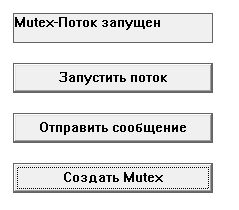
\includegraphics[width=0.7\textwidth]{assets/6.png}\\
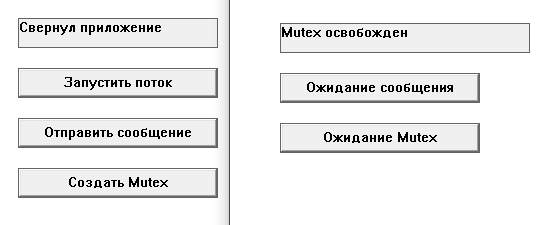
\includegraphics[width=0.7\textwidth]{assets/7.png}\\
\end{center}

Если первое / второе приложение будет закрыто, то нам выпадет ошибка:\\
\begin{center}
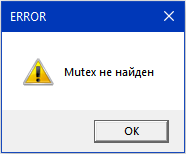
\includegraphics[width=0.4\textwidth]{assets/8.png}
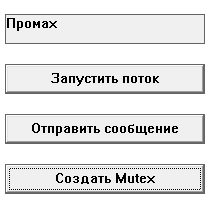
\includegraphics[width=0.4\textwidth]{assets/9.png}\\
\end{center}

При тестировании мы видим корректную работу программы.

\subsection{Создать приложение Windows и добавить в него код создания нового волокна (fiber).}

Определим popup меню для создания дочернего окна:\\
\begin{minted}[fontsize=\footnotesize]{c}
case WM_RBUTTONDOWN:
{
    HMENU hMenu = CreatePopupMenu();
    AppendMenu(hMenu, MF_STRING, IDM_ABOUT, TEXT("О программе"));
    AppendMenu(hMenu, MF_SEPARATOR, 1000, L"");
    AppendMenu(hMenu, MF_STRING, FiberID, TEXT("Создатель волокна"));
    POINT p;
    p.x = LOWORD(lParam);
    p.y = HIWORD(lParam);
    ClientToScreen(hWnd, &p);
    TrackPopupMenu(hMenu, TPM_LEFTALIGN | TPM_TOPALIGN, p.x, p.y, 0, hWnd, NULL);
}
break;

// Добавим в MyRegisterClass дочернее окно.
WNDCLASSEXW child;

child.cbSize = sizeof(WNDCLASSEX);

child.style = CS_HREDRAW | CS_VREDRAW | CS_DBLCLKS;
child.lpfnWndProc = WndProcChild;
child.cbClsExtra = 0;
child.cbWndExtra = 0;
child.hInstance = hInstance;
child.hIcon = NULL;
child.hCursor = LoadCursor(NULL, IDC_ARROW);
child.hbrBackground = (HBRUSH)(COLOR_WINDOW + 1);
child.lpszMenuName = NULL;
child.lpszClassName = _T("ChildWindow");
child.hIconSm = NULL;

RegisterClassExW(&child);
\end{minted}

При создании дочернего окна отрисовываем интерфейс:\\
\begin{minted}[fontsize=\footnotesize]{c}
case FiberID:
    if (!Child1) {
        Child1 = CreateWindow(_T("ChildWindow"), _T("Somethin"), 
            WS_OVERLAPPEDWINDOW | WS_CAPTION | WS_MINIMIZEBOX | WS_VISIBLE | WS_CHILD, 
            600, 0, 300, 300, hWnd, NULL, hInst, NULL);

        FiberBtn = CreateWindow(L"Button", L"Создать волокно", 
            WS_BORDER | WS_VISIBLE | WS_CHILD | BS_PUSHBUTTON, 
            20, 50, 200, 30, Child1, (HMENU)FiberBtnID, hInst, nullptr);
        FOutput = CreateWindow(L"STATIC", L"", WS_BORDER | WS_VISIBLE | WS_CHILD, 20, 80, 200, 30, Child1, NULL, hInst, nullptr);
    }
    ShowWindow(Child1, SW_SHOW);
    UpdateWindow(Child1);
    break;
\end{minted}

Обработчик кнопки дочернего окна:\\
\begin{minted}[fontsize=\footnotesize]{c}
VOID WINAPI FiberFunction2(LPVOID lparam) {
    for (int i = 0; i < 5; i++) {
        SetWindowText(FOutput, L"Пока");
        Sleep(1000);
        SetWindowText(FOutput, L"");
        Sleep(1000);
    }
}

DWORD WINAPI FiberFunction(LPVOID lparam) {
    ConvertThreadToFiber(NULL);
    Fiber2 = CreateFiber(0, FiberFunction2, NULL);
    for (int i = 0; i < 3; i++) {
        SetWindowText(FOutput, L"Привет");
        Sleep(1000);
        SetWindowText(FOutput, L"");
        Sleep(1000);
    }
    SwitchToFiber(Fiber2);
    DeleteFiber(Fiber2);
    ConvertFiberToThread();
    return 0;
}

case FiberBtnID: {
    FiberThread = CreateThread(NULL, 0,
        FiberFunction, NULL, 0, NULL); 
}
\end{minted}

Тестирование:
\begin{center}
При нажатии правой кнопки мыши мы видим меню:\\

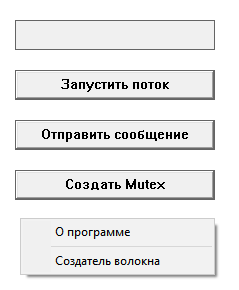
\includegraphics[width=0.4\textwidth]{assets/10.png}\\

После нажатия на кнопку "Создатель волокна" у нас открывается дочернее окно:\\

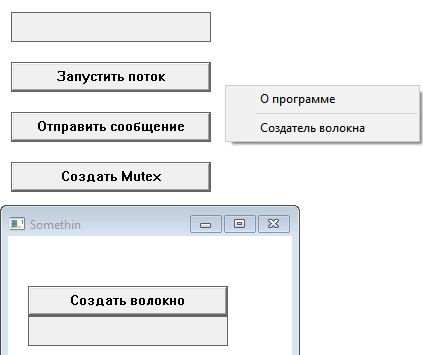
\includegraphics[width=0.6\textwidth]{assets/11.png}\\

После нажатия на "Создать волокно" у нас выведется 3 раза привет и 5 раз пока:\\

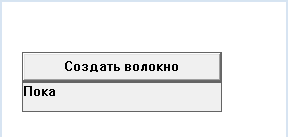
\includegraphics[width=0.4\textwidth]{assets/13.png}\\

\end{center}
Итог: При работе с потоками планировщиком выступает компилятор, а вот волокно планируется полностью вручную.

\end{document}

